\documentclass[12pt,a4paper]{report}
\usepackage{amsmath}
\usepackage{ucs}
\usepackage[utf8x]{inputenc}
\usepackage{indentfirst}
\usepackage[greek,english]{babel}
\newcommand{\en}{\selectlanguage{english}}
\newcommand{\gr}{\selectlanguage{greek}}
\newcommand{\HRule}[1]{\rule{\linewidth}{#1}}
\usepackage{listings}
\usepackage{graphicx}
\usepackage{float}
\usepackage{subcaption}

\title{ \normalsize \textsc{}
		\\ [2.0cm]
		\HRule{0.5pt} \\
		\LARGE \text{\gr Αναφορά Υπολογιστικής Εργασίας}
		\LARGE \text{\gr στο μάθημα των Χρονοσειρών}
		\HRule{0.5pt} \\ [0.5cm]
		\normalsize \vspace*{5\baselineskip}
		}
	
\author{
  \gr Ζήσου Χαρίλαος\\
  \text{\gr ΑΕΜ: 9213}
  \and
  \gr Καρατζάς Μιχάλης\\
  \text{\gr ΑΕΜ: 9137}
}

\date{}

\begin{document}
\maketitle
\newpage
\begin{center}
\LARGE \textbf{\gr Ανάλυση ιστορικών δεδομένων ηλεκτρικής ενέργειας της Ιταλίας}
\end{center}

\section{\gr Γραμμική ανάλυση}
\gr Η ομάδα μας είχε τον αριθμό 7, επομένως κληθήκαμε να αναλύσουμε δεδομένα στις 08:00 η ώρα για όλη την επικράτεια. Η ανάλυση χωρίστηκε σε 2 αρχεία στο \en matlab \gr ξεχωριστά για \en demand \gr και \en price, \gr κάθε ένα από τα οποία περιέχει τη γραμμική και μη γραμμική μελέτη.

\subsection{\gr Τάση και περιοδικότητα}
Όσον αφορά την τάση, δοκιμάζοντας προσαρμογή με πολυώνυμο και \en moving average \gr φίλτρο, δεν μείναμε ικανοποιημένοι από τα αποτελέσματα και αποφασίσαμε να χρησιμοποιήσουμε τις πρώτες διαφορές, λαμβάνοντας έτσι μια χρονοσειρά εντελώς απαλαγμένη από την τάση.

\begin{figure}[H]
\begin{subfigure}{0.5\textwidth}
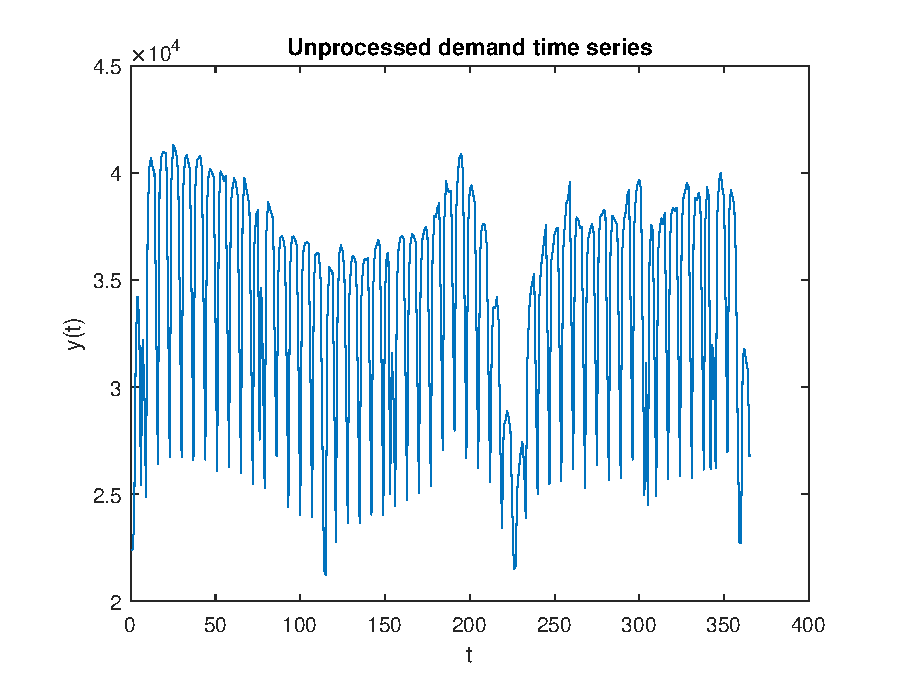
\includegraphics[width=\linewidth]{unprocessedDemand.eps} 
\end{subfigure}
\begin{subfigure}{0.5\textwidth}
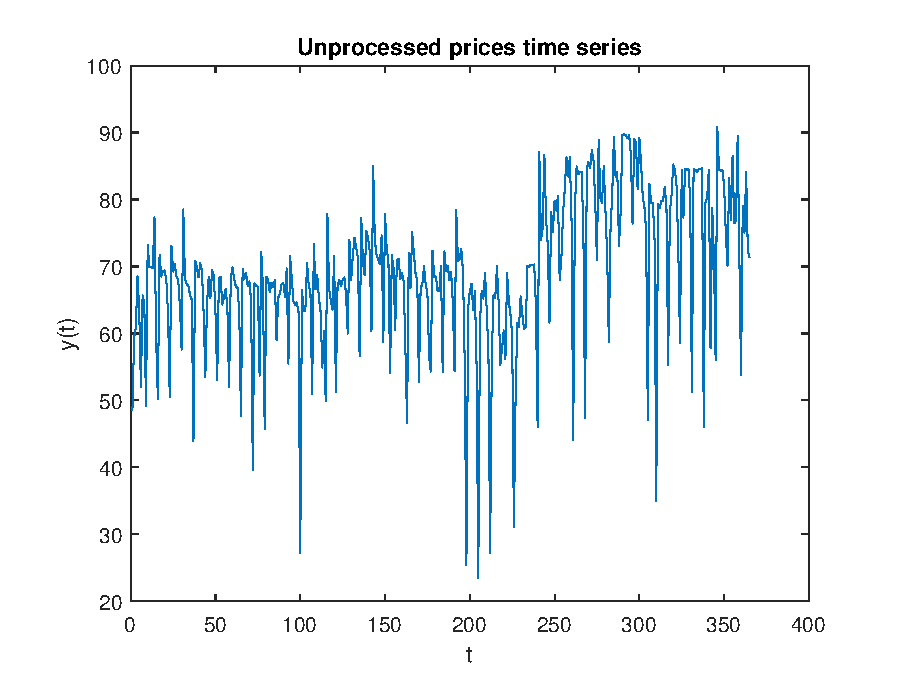
\includegraphics[width=\linewidth]{unprocessedPrices.eps}
\end{subfigure}
\end{figure}


\begin{figure}[H]
\begin{subfigure}{0.5\textwidth}
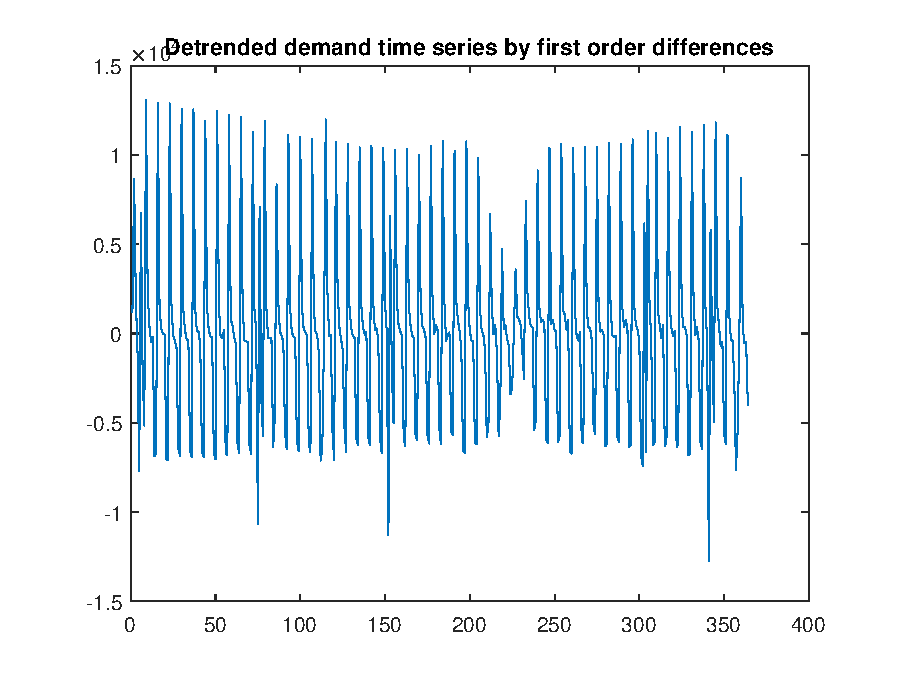
\includegraphics[width=\linewidth]{detrendedDemand.eps} 
\end{subfigure}
\begin{subfigure}{0.5\textwidth}
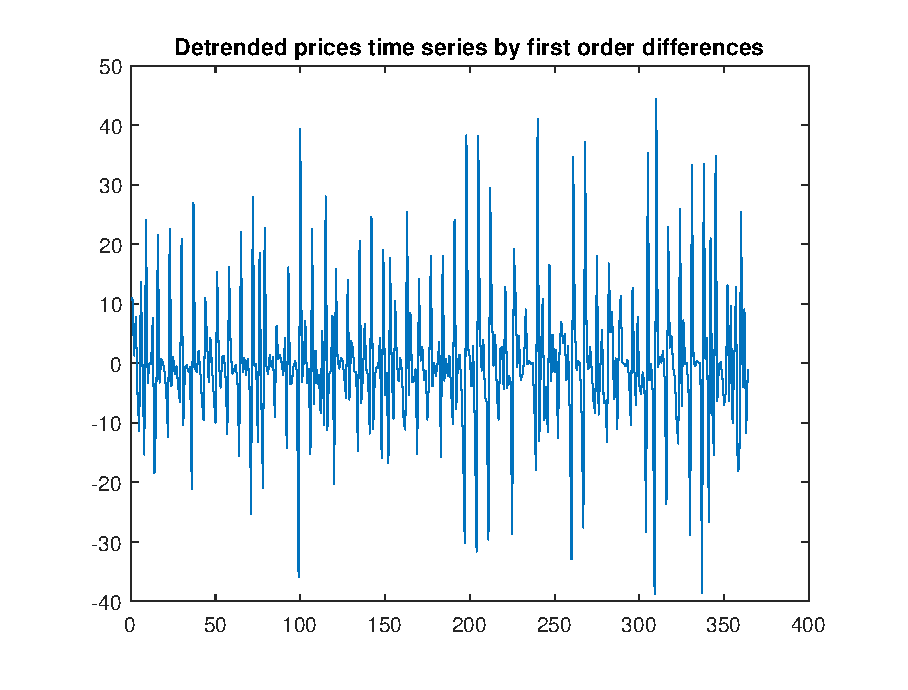
\includegraphics[width=\linewidth]{detrendedPrices.eps}
\end{subfigure}
\end{figure}

Για την περιοδικότητα χρησιμοποιήσαμε τη συνάρτηση \en seasonalcomponents \gr με περίοδο 7, στοχεύοντας στην αφαίρεση του εβδομαδιαίου κύκλου

\begin{figure}[H]
\begin{subfigure}{0.5\textwidth}
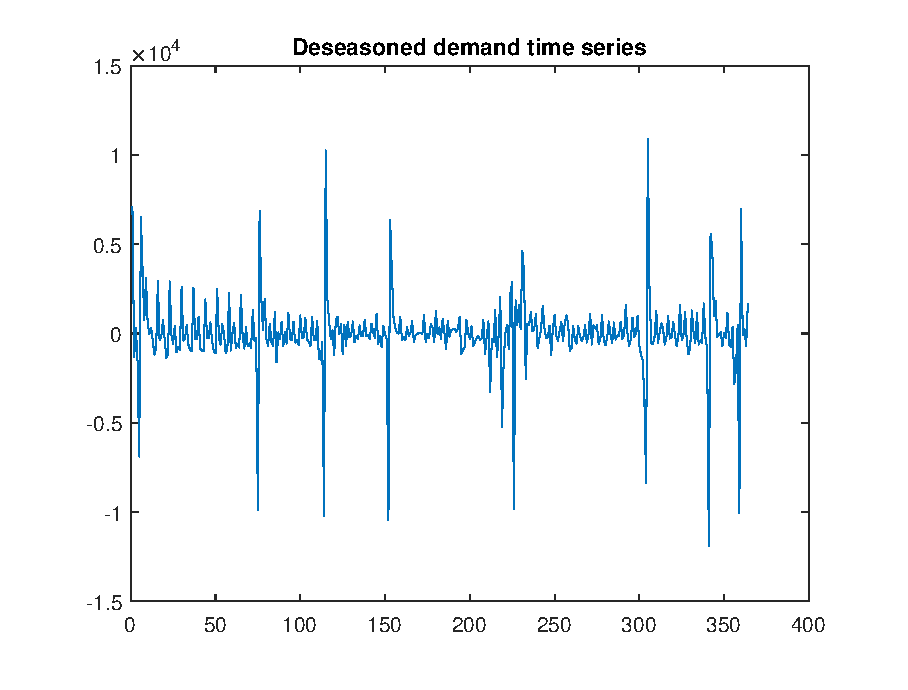
\includegraphics[width=\linewidth]{deseasonedDemand.eps} 
\end{subfigure}
\begin{subfigure}{0.5\textwidth}
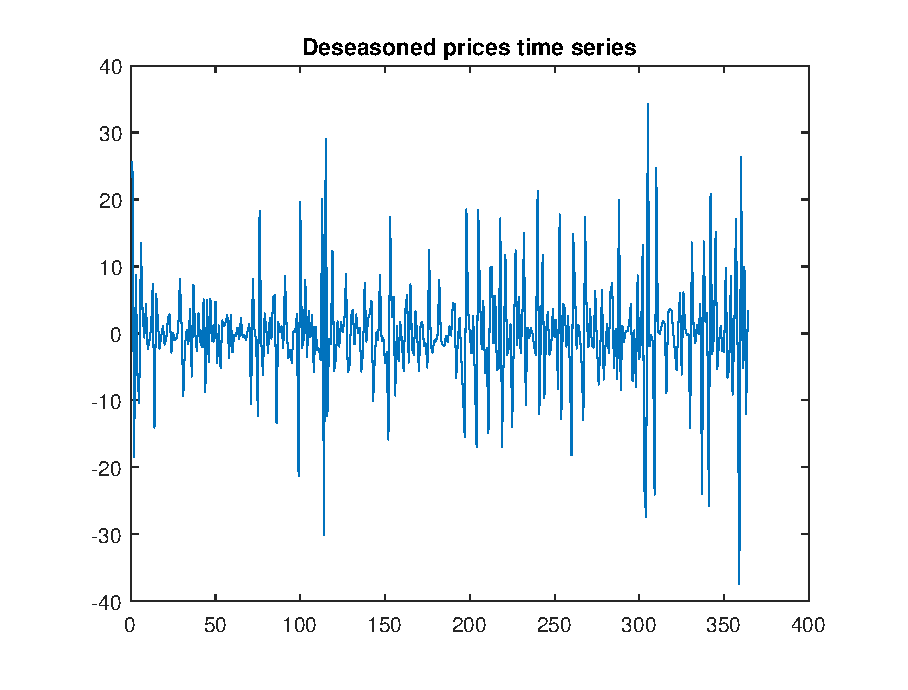
\includegraphics[width=\linewidth]{deseasonedPrices.eps}
\end{subfigure}
\end{figure}

\subsection{\gr Συνάρτηση αυτοσυσχέτισης - Έλεγχος λευκού θορύβου}

\begin{figure}[H]
\begin{subfigure}{0.5\textwidth}
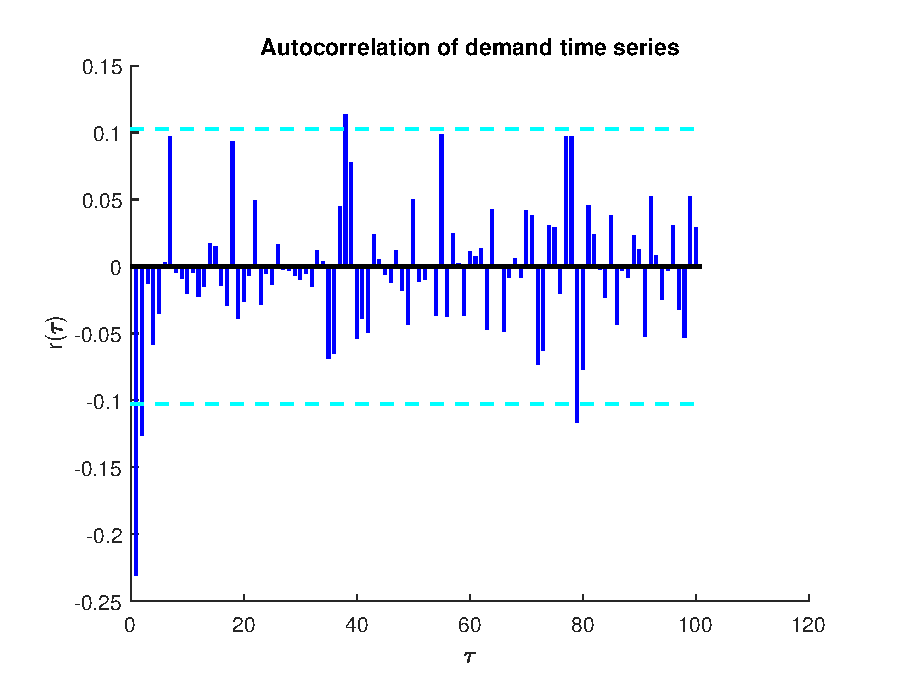
\includegraphics[width=\linewidth]{acDemand.eps} 
\end{subfigure}
\begin{subfigure}{0.5\textwidth}
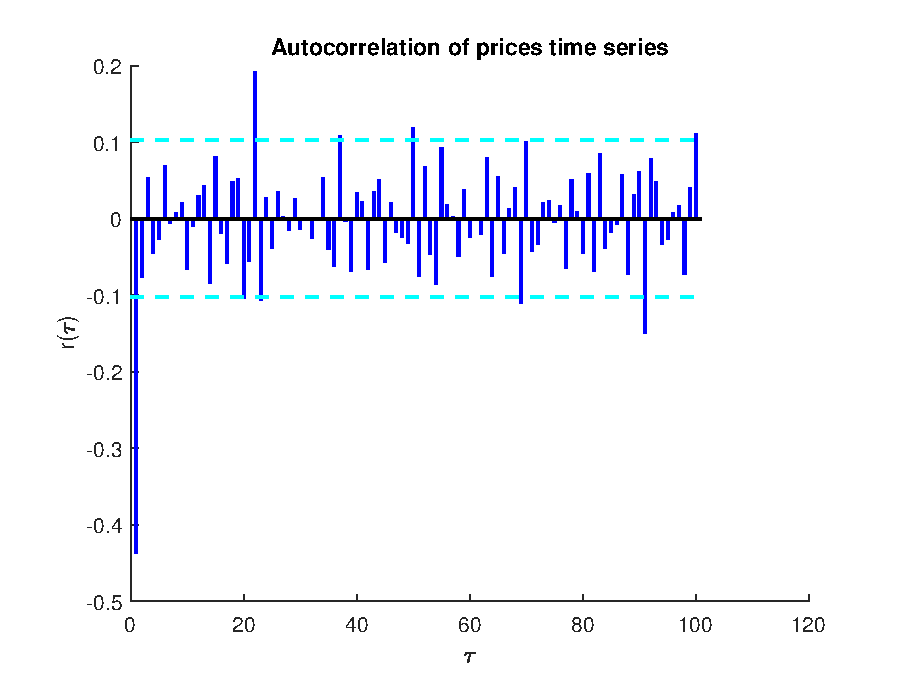
\includegraphics[width=\linewidth]{acPrices.eps}
\end{subfigure}
\end{figure}

\begin{figure}[H]
\begin{subfigure}{0.5\textwidth}
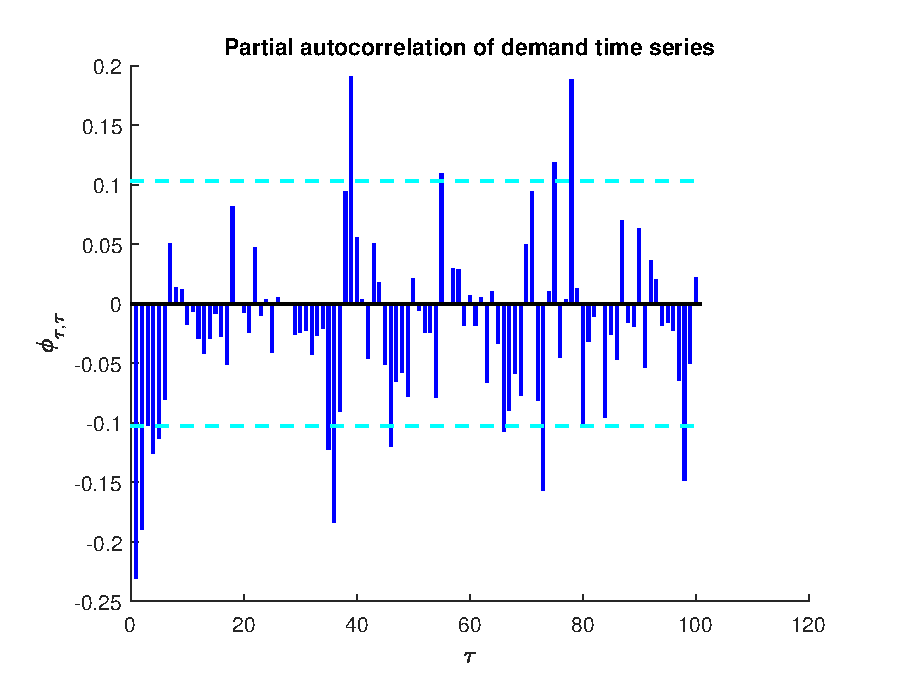
\includegraphics[width=\linewidth]{pacDemand.eps} 
\end{subfigure}
\begin{subfigure}{0.5\textwidth}
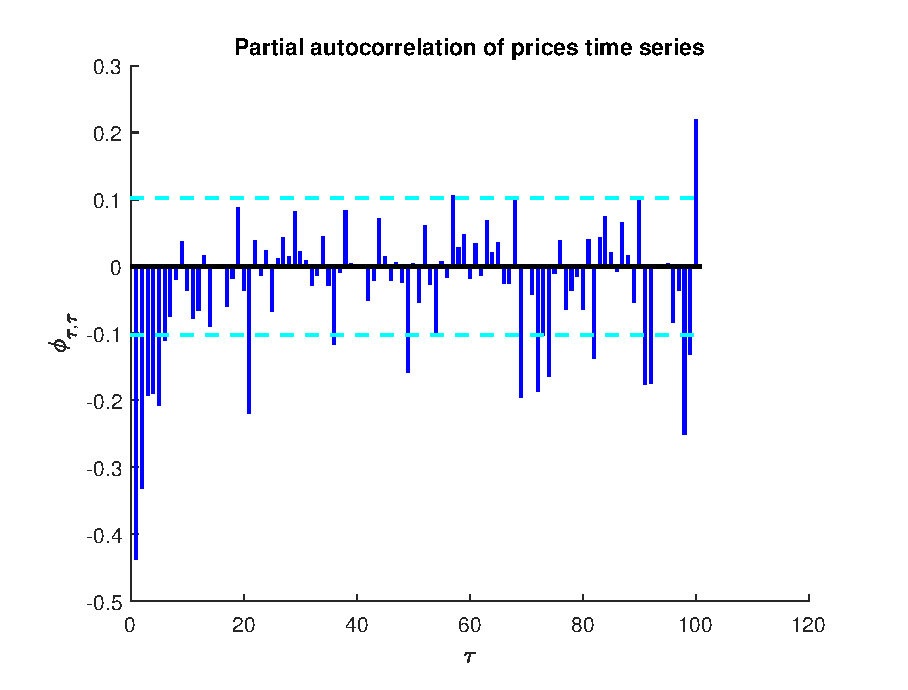
\includegraphics[width=\linewidth]{pacPrices.eps}
\end{subfigure}
\end{figure}

Λόγω των αυτοσυσχετίσεων για $\tau=1,2$ και $\tau=1$ αντίστοιχα, αλλά και για άλλες τιμές που ξεπερνούν τα όρια σημαντικότητας, δεν μπορώ να θεωρήσω πως η χρονοσειρά που απομένει είναι λευκός θόρυβος. Μάλιστα ένα πιο σωστό τεστ που θα μπορούσαμε να κάνουμε είναι το \en Ljung-Box Portmanteau test \gr το οποίο δίνεται παρακάτω:

\begin{figure}[H]
\begin{subfigure}{0.5\textwidth}
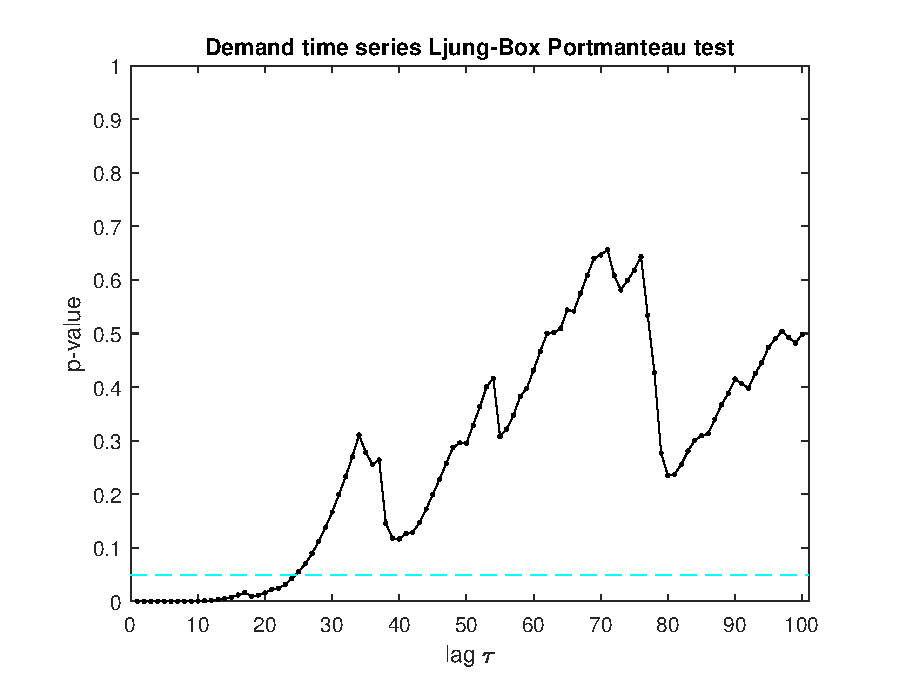
\includegraphics[width=\linewidth]{lbDemand.eps} 
\end{subfigure}
\begin{subfigure}{0.5\textwidth}
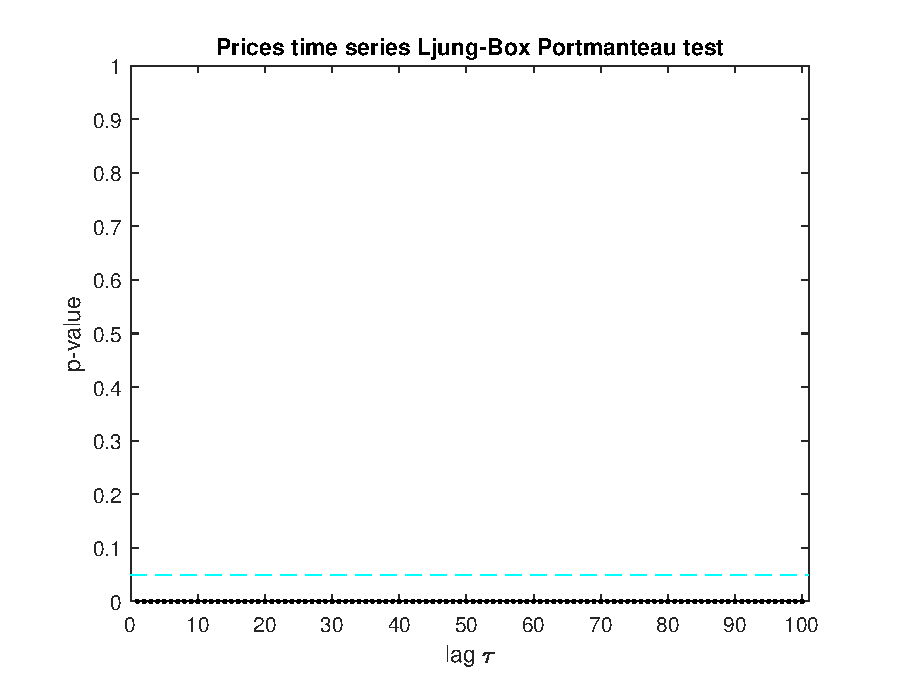
\includegraphics[width=\linewidth]{lbPrices.eps}
\end{subfigure}
\end{figure}

Και από αυτό το τεστ συμπεραίνουμε πως το επίπεδο $p=0.05$ δεν ξεπερνιέται παρα μόνο για μεγάλες υστερήσεις στην μια περίπτωση και καθόλου στην άλλη, επομένως μπορούμε να απορρίψουμε την μηδενική υπόθεση ότι οι χρονοσειρές είναι λευκός θόρυβος και άρα έχει νόημα να προχωρήσουμε στο επόμενο βήμα και να προσπαθήσουμε να προσαρμόσουμε κάποιο γραμμικό μοντέλο.

\subsection{\gr Προσαρμογή γραμμικού μοντέλου \en ARMA}
Σύμφωνα με τη θεωρία, για την επιλογή ενός κατάλληλου μοντέλου \en ARMA \gr δεν μπορούμε να βασιστούμε στις συναρτήσεις αυτοστυσχέτισης η μερικής αυτοσυσχέτισης, αλλά πρέπει να υπολογίσουμε κάποιο άλλο κριτήριο όπως το κριτήριο του \en Akaike (AIC) \gr που χρησιμοποιήσαμε εμείς.

\begin{figure}[H]
\begin{subfigure}{0.5\textwidth}
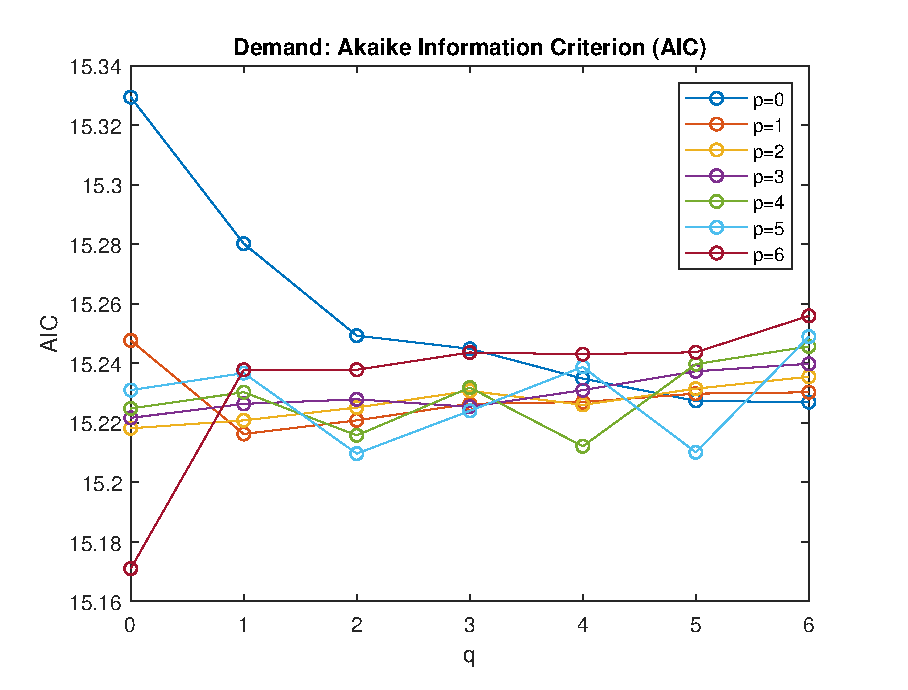
\includegraphics[width=\linewidth]{aicDemand.eps} 
\end{subfigure}
\begin{subfigure}{0.5\textwidth}
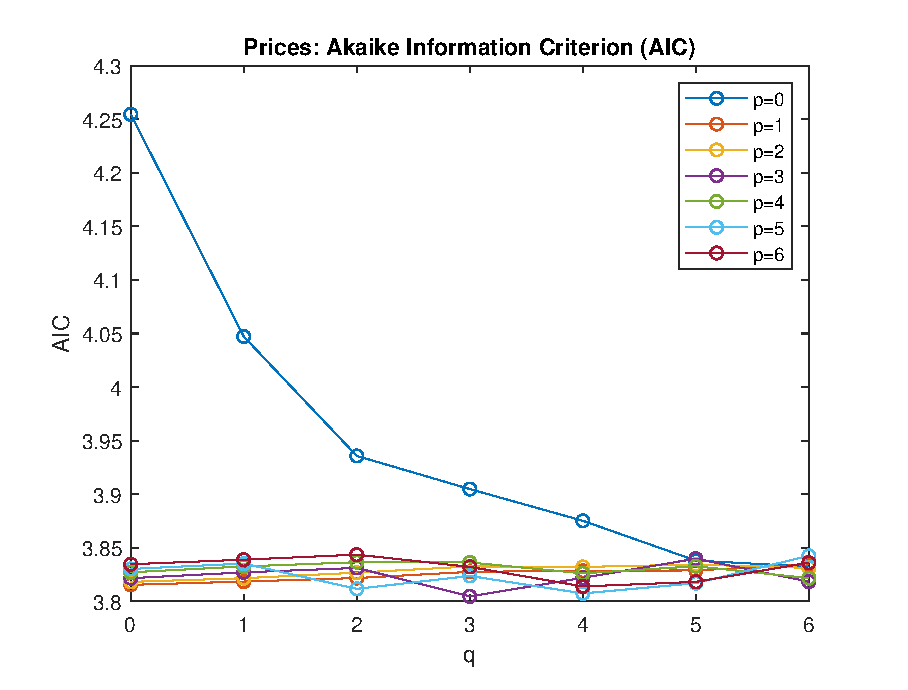
\includegraphics[width=\linewidth]{aicPrices.eps}
\end{subfigure}
\end{figure}

Επομένως, τα μοντέλα που χρησιμοποιήσαμε ήταν $ARMA(0,6)$ για \en demand time series \gr και $ARMA(3,3)$ για \en prices time series\gr , καθώς ήταν αυτά που πετυχαίνανε το χαμηλότερο κριτήριο. Τα σφάλματα που παράγουν τα μοντέλα για έως και 10 βήματα μπροστά, δίνονται παρακάτω:

\begin{figure}[H]
\begin{subfigure}{0.5\textwidth}
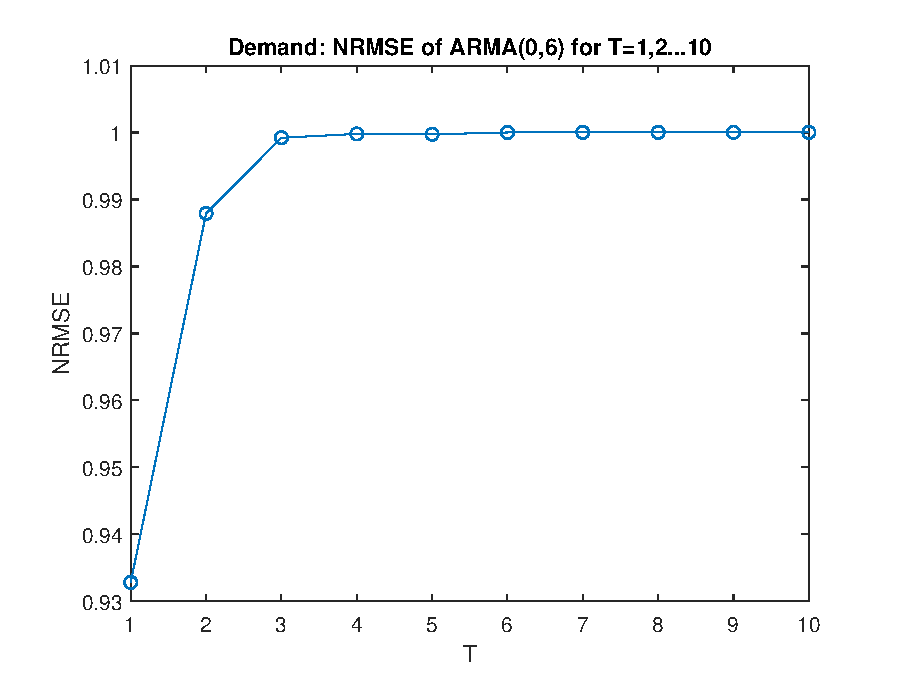
\includegraphics[width=\linewidth]{nrmseARMADemand.eps} 
\end{subfigure}
\begin{subfigure}{0.5\textwidth}
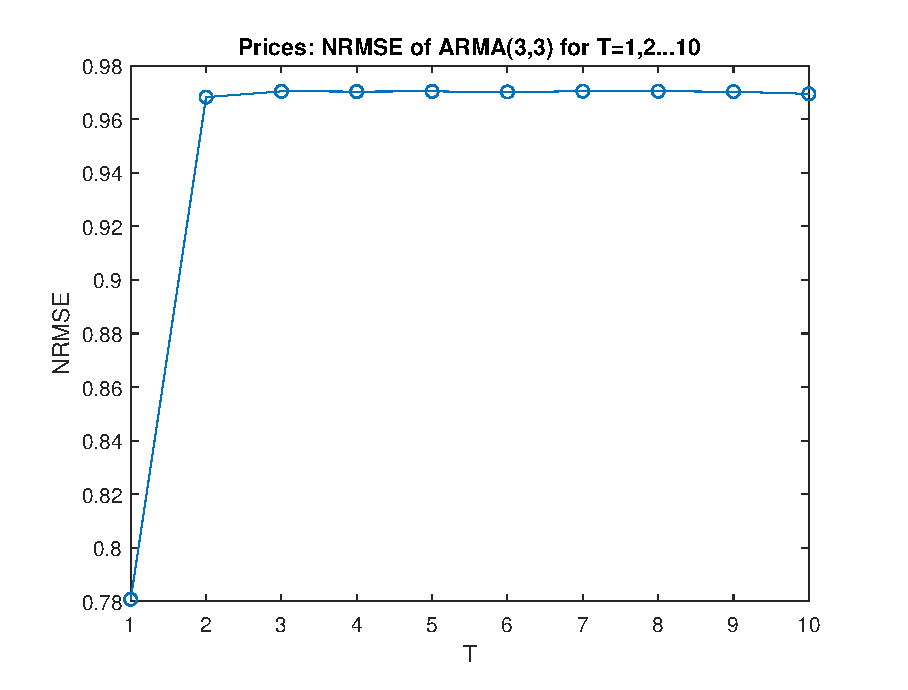
\includegraphics[width=\linewidth]{nrmseARMAPrices.eps}
\end{subfigure}
\end{figure}

Με βάση όλα τα παραπάνω, παρατηρούμε πως οι χρονοσειρές ζήτησης και τιμής έχουν παρόμοιες συναρτήσεις αυτοσυσχέτισης και μερικής αυτοσυσχέτισης, και πως καμία από τις 2 δεν μπορεί να θεωρηθεί λευκός θόρυβος. Ωστόσο τα μοντέλα που προσαρμόσαμε φαίνεται να διαφέρουν, αν και έχουν ένα σχετικά παρόμοιο σφάλμα προσαρμογής, $0.93$ για \en demand \gr και λίγο καλύτερο $0.78$ για \en prices, \gr τα οποία φυσικά τείνουν στην μονάδα καθώς αυξάνονται τα βήματα.

\subsection{\gr Προβλέψεις επόμενης ημέρας}
Για τις προβλέψεις της επόμενης ημέρας σπάσαμε τις χρονοσειρές σε 5 διακριτά σημεία ώστε να χρησιμοποιούμε πχ το $70\%$ των δεδομένων ως \en training data \gr  και τα υπόλοιπα ως \en validation data.\gr

\begin{figure}[H]
\begin{subfigure}{0.5\textwidth}
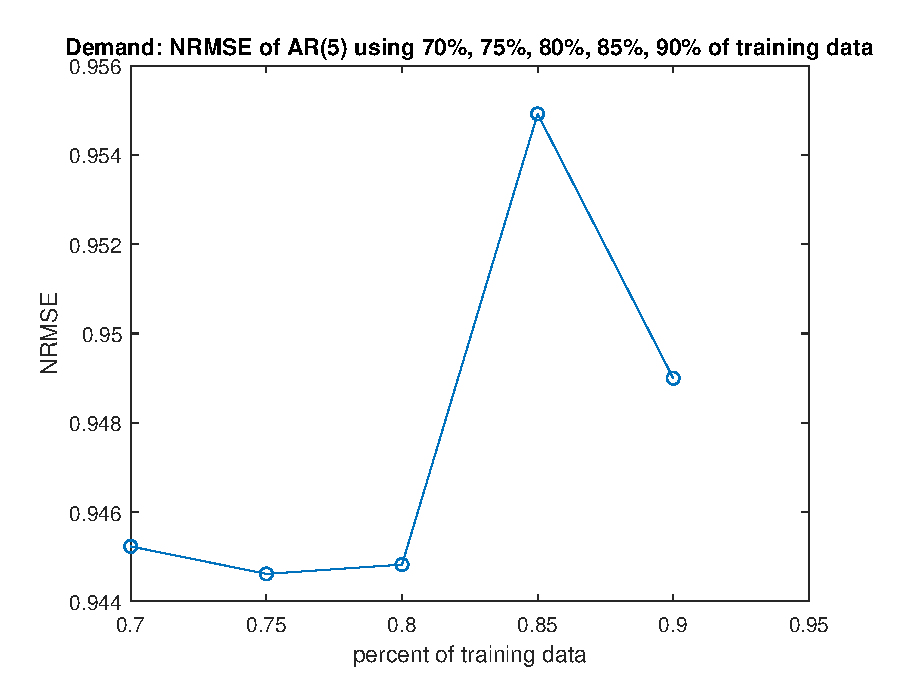
\includegraphics[width=\linewidth]{nrmseDemand.eps} 
\end{subfigure}
\begin{subfigure}{0.5\textwidth}
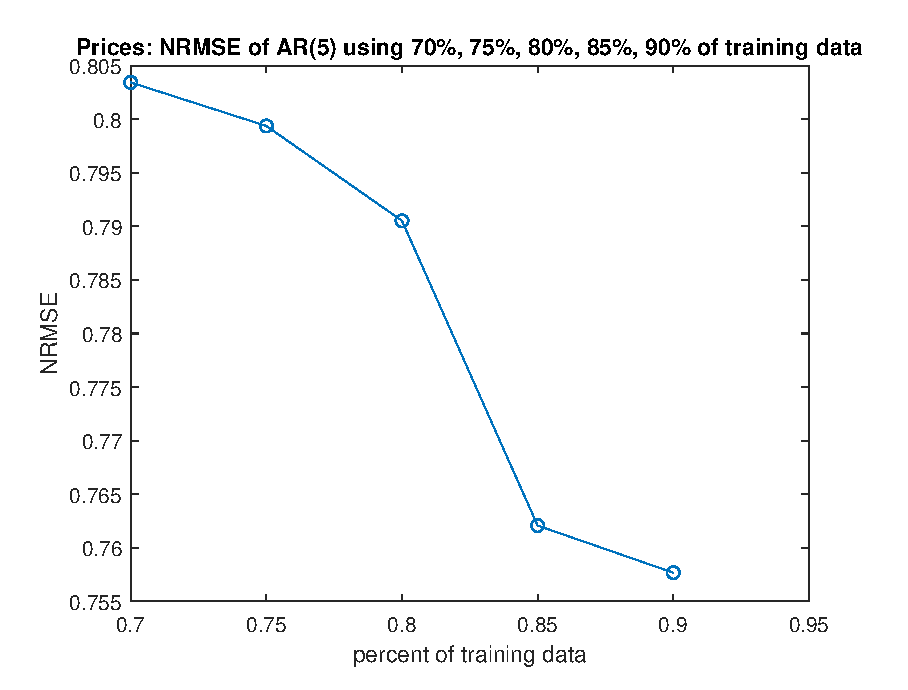
\includegraphics[width=\linewidth]{nrmsePrices.eps}
\end{subfigure}
\end{figure}

Καθώς μετακινούμε το σημείο του διαχωρισμού, παρατηρούμε πως δεν συμπίπτει το χαμηλότερο \en NRMSE \gr για τις 2 χρονοσειρές. Στη χρονοσειρά της ζήτησης, καθώς αυξάνεται το σύνολο εκμάθησης, αυξάνεται και το σφάλμα πρόβλεψης, γεγονός που υποδηλώνει \en over-fitting \gr ενώ στη χρονοσειρά των τιμών, παρατηρούμε πως συνεχώς μειώνεται.

\section{\gr Μη-γραμμική ανάλυση}
\subsection{\gr Εκτίμηση γραμμικών και μη γραμμικών στατιστικών}

\end{document}